\section{Optimal Control of Pitch/Travel and Elevation with and without Feedback}\label{sec:prob4}
\label{text:problem4}

The 

\subsection{State space model}
We wish to calculate an optimal trajectory in two dimension, adding a constraint to the elevation. Adding $e$ and $\dot{e}$ to the previous state space model \eqref{eq:sys} and using \eqref{eq:e_ec}, we get
\begin{equation}
	\begin{bmatrix}
		\dot{\lambda}\\
		\ddot{\lambda}	\\
		\dot{p}	\\
		\ddot{p}\\
		\dot{e}	\\
		\ddot{e}
	\end{bmatrix} = 
	\underbrace{
	\begin{bmatrix}
		0 & 1 & 0 & 0 & 0  & 0 \\
		0 & -0.03 & -0.39 & 0 & 0 & 0 \\
		0 & 0 & 0 & 1 & 0 & 0 \\
		0 & 0 & -7.13 & -3.6 & 0 & 0 \\
		0 & 0 & 0 & 0 & 0 & 1 \\
		0 & 0 & 0 & 0 & -3.03 & -2.44 \\
	\end{bmatrix}}_{A_c}
	\begin{bmatrix}
		\lambda	\\
		\dot{\lambda}\\
		p		\\
		\dot{p} \\
		e		\\
		\dot{e}
	\end{bmatrix} +
	\underbrace{
	\begin{bmatrix}
		0 & 0\\
		0 & 0\\
		0 & 0\\
		6.74 & 0\\
		0 & 0 \\
		0 & 3.13 \\
	\end{bmatrix}}_{B_c}
	\begin{bmatrix}
	p_c \\
	e_c
	\end{bmatrix}
	\label{eq:ex_sys}
\end{equation}

The added states are clearly decoupled from the rest of the system. This is due to the fact that the model is linearized around the equilibrium. At small pitch angles this simplification does not cause any large discrepancies. However, when the pitch angle is large, an increase in elevation rate is clearly accompanied by an increase in travel rate. 

\subsection{Discretization}
Now let $x = \begin{bmatrix}\lambda&\dot{\lambda}&p&\dot{p}&e&\dot{e}\end{bmatrix}^\top$, $u = \begin{bmatrix}p_c&e_c\end{bmatrix}^\top$. Again, using approximate discretization via Euler we obtain a discrete state space model
\begin{subequations}
\begin{align}
	\label{eq:ex_dsys}
	x_{k+1} &= (I + \Delta t A_c) x_k + (\Delta t B_c) u_k. \\
	&= Ax_k + Bu_k,
\end{align}
\end{subequations}

where 
\begin{equation*}
	A = 
	\begin{bmatrix}
		1 & 0.25 & 0 & 0 & 0 & 0\\
		0 & 0.9925 & -0.0975 & 0 & 0 & 0\\
		0 & 0 & 1 & 0.25 & 0 & 0\\
		0 & 0 & -1.7825 & 0.1 & 0 & 0\\
		0 & 0 & 0 & 0 & 1 & 0.25\\
		0 & 0 & 0 & 0 & -0.7575 & 0.39
	\end{bmatrix}, \quad
	B = 
	\begin{bmatrix}
		0 & 0\\
		0 & 0\\
		0 & 0\\
		1.685 & 0\\
		0 & 0\\
		0 & 0.7825
	\end{bmatrix}.
\end{equation*}

\subsection{Optimization problem with nonlinear constraints}

We calculate an optimal trajectory from $x_0 = \begin{bmatrix}\lambda_0&0&0&0&0&0\end{bmatrix}^\top$ to $x_f = \begin{bmatrix}\lambda_f&0&0&0&0&0\end{bmatrix}^\top$ minimizing the objective function 
\begin{equation*}
	\phi = \sum_{i=1}^{N}(\lambda_i - \lambda_f)^2 + r_1 p^2_{c_i} + r_2 e^2_{c_i}, \quad r_1,r_2 \ge 0,
\end{equation*}

or alternatively
\begin{equation}
	\label{eq:quad_cost}
	\phi = \sum_{i=0}^{N-1} (x_{i+1}-x_f)^\top Q(x_{i+1}-x_f) + u_i^\top R u_i,
\end{equation}
where

\begin{equation}
Q = \begin{bmatrix}1&0&0&0&0&0\\0&0&0&0&0&0\\0&0&0&0&0&0\\0&0&0&0&0&0\\0&0&0&0&0&0\\0&0&0&0&0&0\end{bmatrix}, \quad R = \begin{bmatrix}r_1&0\\0&r_2\end{bmatrix}.
\end{equation}

 The second weighting parameter $r_2$ is added as we impose an inequality constraint on the elevation for every time step:

\begin{equation}
	\label{eq:cons}
	c(x_k) = \alpha \exp{\left(-\beta\left(\lambda_k - \lambda_t\right)^2\right)} - e_k \le 0, \quad k = \{1, \dots , N\},
\end{equation}
where we let $\alpha = 0.2$, $\beta = 20$, $\lambda_t = \frac{2\pi}{3}$.

The objective function \eqref{eq:quad_cost} is subject to the system dynamics \eqref{eq:ex_dsys} and thus imposed to linear equality constraints identically defined to that of \eqref{eq:eq_constraints}. Similarly to \eqref{eq:QP_travel} we define the optimization variable $z$ and the matrix $G$, and the resulting optimization problem can be stated:
\begin{subequations}
\label{eq:NOP}
	\begin{equation}
		\min_z \quad z^T G z
	\end{equation}
subject to
\begin{align}
	A_{eq} z &= B_{eq}, \\
	c(x_k) &\le 0, \quad k = \{1, \dots N\},\\
	p^{\textrm{low}} \le p_k &\le p^{\textrm{high}}, \quad k = \{1, \dots N\}.
\end{align}
\end{subequations}


\subsection{Discrete LQR}
In addition to running the optimal input sequence $u^*$ in an open loop, a discrete LQ-controller is applied, with the weigthing matrices

\begin{equation}
Q = \begin{bmatrix}4&0&0&0&0&0\\0&2&0&0&0&0\\0&0&0&0&0&0\\0&0&0&0&0&0\\0&0&0&0&3&0\\0&0&0&0&0&0\end{bmatrix}, \quad R = \begin{bmatrix}1&0\\0&1\end{bmatrix}.
\end{equation}
\subsection{Optional: Additional constraints}
\label{text:additionalContraints}

Although the calculated input yielded satisfactory performance, the model has shortcomings. Specifically, when a low decent in elevation is commanded the rotor blades almost come to a complete stop, during which control of pitch is severely reduced. As this is impossible to model with a linear model, additional bounds are imposed on elevation rate. This will reduce the effect of the unmodeled coupling of elevation to the rest of the system. In a further attempt to keep the system within the linear area the travel rate is also bounded. The bounds are

\begin{align*}
	|\dot{e_k}| &\le 0.05, \\
	|\dot{\lambda_k}| &\le 0.5.
\end{align*}
\subsection{Results and discussion}

 Because of the non-linearity of \eqref{eq:cons} it is no longer viable to use a QP-solver, and \eqref{eq:NOP} is solved using MATLAB's \texttt{fmincon} which uses an active set method. The pitch bounds are also tightened from $45$ to $25$ degrees in order to lower the effect of elevation rate and travel rate coupling at large pitch angles. 

The optimal input sequence $u^*$ is applied to the plant in an open loop with results shown in figure \ref{fig:openloop25}. The system follows the optimal trajectory except for the usual discrepancy in travel present when using open loop control. We further employ an LQ-controller similar to in \ref{text:LQR} to guide the trajectory to the set-point and eliminate steady state deviations. The result, shown in figure \ref{fig:closedloop25}, is without any large discrepancies between optimal and measured trajectory. However, the constraint bound imposed on elevation is violated, as shown in figure \ref{fig:closedloop25_cons}. The reason for this is probably a combination of issues. The optimal path is calculated with a fairly large time step, in order to lower the computational time required. This leads to an optimal path that when interpolated will violate the constraint. Also, as the increase in elevation will largely happen when the pitch angle is at its maximum, and the resulting increase in elevation will be lower than if the increase were to be commanded at zero pitch. State feedback is also unable to deal with this problem completely, as any aggressive elevation correction is bound to happen at the cost of pitch, and therefore travel rate control. Lastly, the trajectory is corrected with respect to the optimal path in time, while the bound on elevation is defined with respect to travel. This means that a deviation in travel, as visible in figure \ref{fig:closedloop25}, effectively will shift the optimal elevation path with respect to travel. This lag is visible in figure \ref{fig:closedloop25_cons}.

The mentioned effects contributing to constraint violation are attempted minimized by the addition of extra constraints on elevation rate and travel rate, as mentioned in \ref{text:additionalContraints}. The resulting optimal path reflects this, and the slope of the optimal elevation path is significantly reduced. This yields an overall less aggressive system, with decreased violation of the elevation constraint. The added constraint on travel rate also means that the system uses the entire time slot to reach the desired end state.

\begin{figure}[hp]
	\centering
		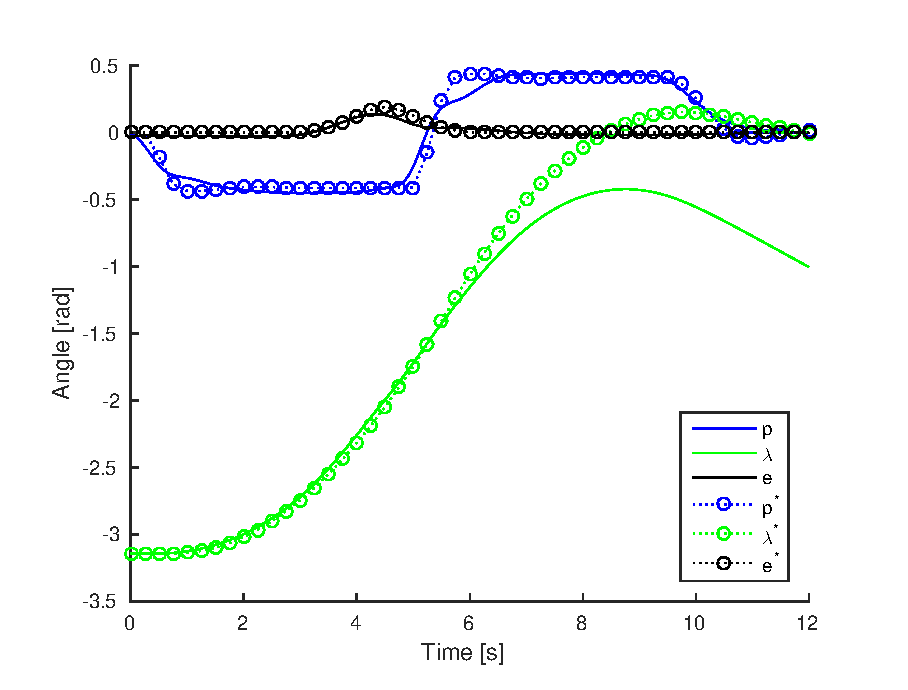
\includegraphics[width=0.85\textwidth]{figures/4/openloop25.eps}
	\caption{Open Loop 25.}
	\label{fig:openloop25}
\end{figure}

\begin{figure}[hp]
	\centering
		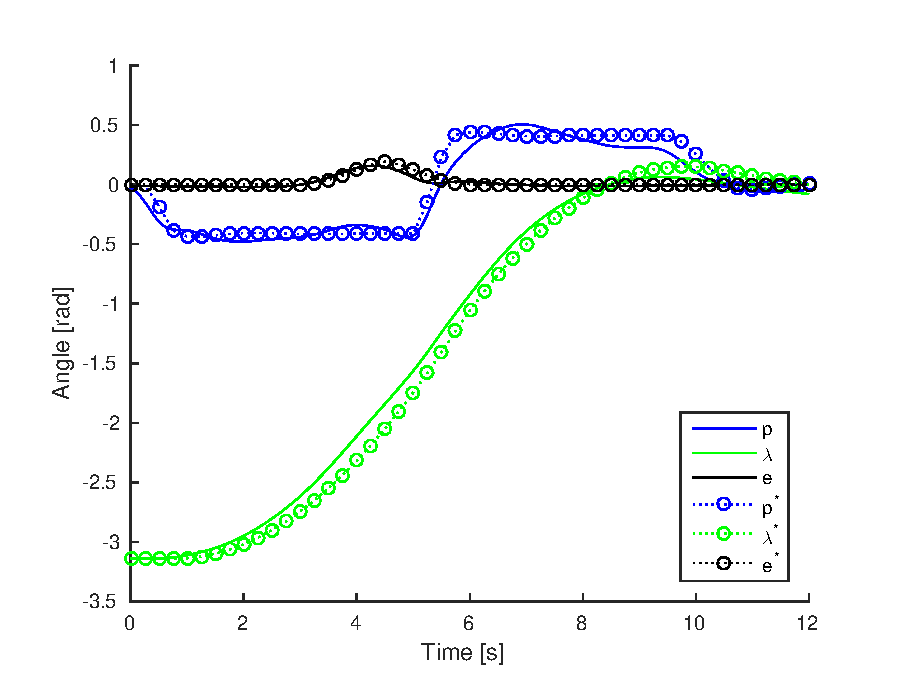
\includegraphics[width=0.85\textwidth]{figures/4/closedloop25.eps}
	\caption{Closed Loop 25.}
	\label{fig:closedloop25}
\end{figure}

\begin{figure}[hp]
	\centering
		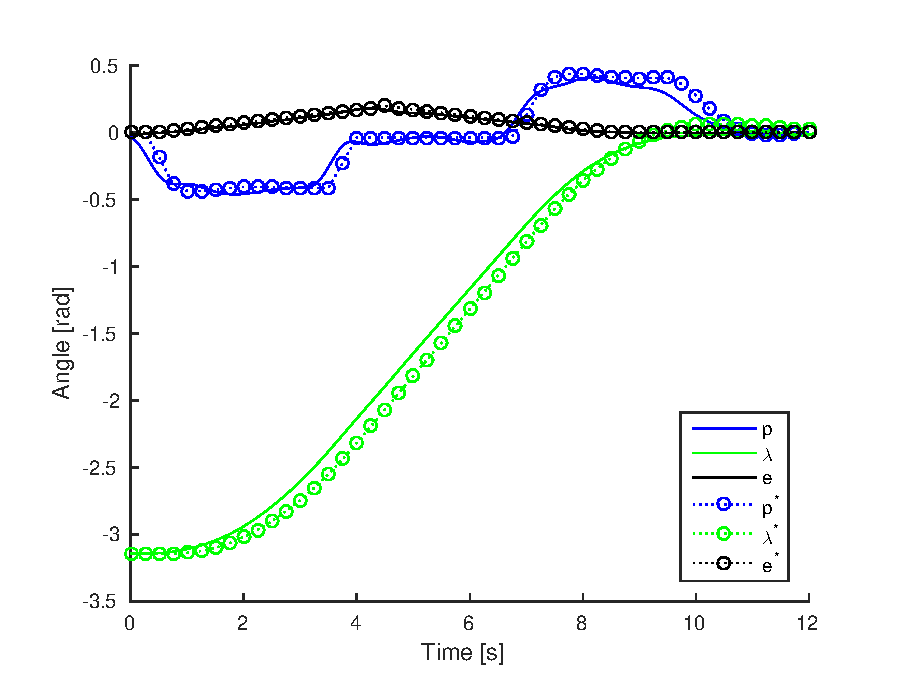
\includegraphics[width=0.85\textwidth]{figures/4/closedloopConstrained25.eps}
	\caption{Closed Loop 25, extra constraints.}
	\label{fig:closedloopConstrained25}
\end{figure}

\begin{figure}[hp]
	\centering
		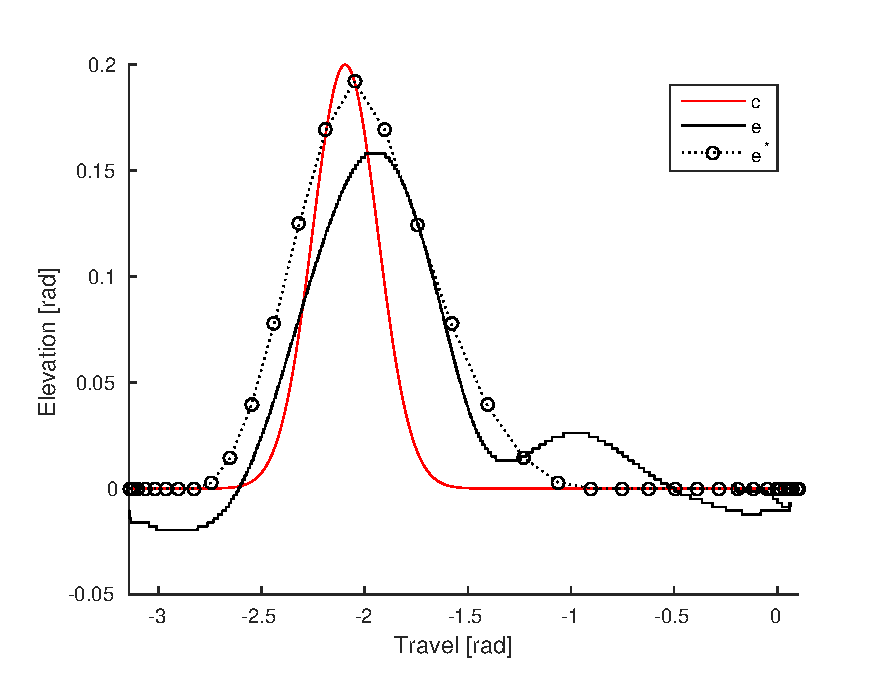
\includegraphics[width=0.85\textwidth]{figures/4/closedloop25_cons.eps}
	\caption{Closed Loop 25 - contraint hill.}
	\label{fig:closedloop25_cons}
\end{figure}

\begin{figure}[hp]
	\centering
		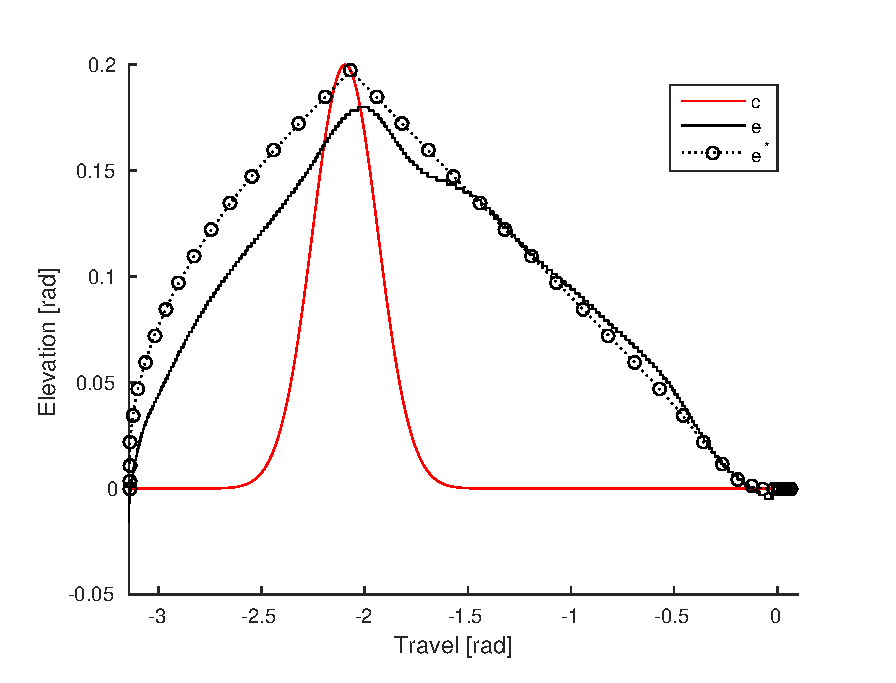
\includegraphics[width=0.85\textwidth]{figures/4/closedloopConstrained25_cons.eps}
	\caption{Closed Loop 25, extra constraints - contraint hill.}
	\label{fig:closedloopConstrained25_cons}
\end{figure}

